%\documentclass[12pt,preprint]{aastex}
%\documentclass[preprint2,12pt]{aastex}
\documentclass{emulateapj}
%\usepackage{apjfonts}
\usepackage{graphicx}
\usepackage{amssymb}
\usepackage{amsmath}
\usepackage{todonotes}

\shortauthors{LGB, KM, JNW}
\shorttitle{Toy transit surveys}

\begin{document}

% ------------------------------------------------------------------------
% New commands
%
\def\ltsima{$\; \buildrel < \over \sim \;$}
\def\lsim{\lower.5ex\hbox{\ltsima}}
\def\gtsima{$\; \buildrel > \over \sim \;$}
\def\gsim{\lower.5ex\hbox{\gtsima}}
\def\tess{{\it TESS} }
\def \teff {T_{\rm eff}}
\def \phir {\Phi_{\rm R}}
\def \fov {24$^{\circ}$}
\def \pixsz {21.1''}
\def \aeff {69.1 cm$^2$ }    
\def \epd {105 mm}                          
                                                                                          
% -------------------------------------------------------------------------
%

\bibliographystyle{apj}

\title{ Analytic Transit Surveys }

\author{
  LGB, KM, JNW
}

% \journalinfo{Draft version}
\slugcomment{Memo for internal use}

%\altaffiltext{1}{Princeton University}

\begin{abstract}

We describe a few different toy transit surveys.

First, we derive the signal to noise distribution of planets detected in a 
survey where all the stars and planets are the same (except some stars are twin 
binary systems). We give expressions for the number of detected planets, and 
for possible errors one can make when deriving occurrence rates.

Then, we allow the properties of the secondary in binary systems to vary. A 
distribution of light ratios introduces additional biases, which we discuss.
We reassess the errors related to occurrence rates.


\end{abstract}

\keywords{planets and satellites:\ detection}

\section{Model \#1: fixed stars, fixed planets, fixed light-ratio binaries}
\label{sec:model_1}

Ah, transiting planets! We learn so much by studying them. But how much can we 
actually learn, and how much is messed up by binarity?

Imagine the following transit survey:
\begin{enumerate}
\item You are going to observe the entire sky for a duration $T_{\rm obs}$, 
with a detector of area $A$, and known bandpass. Your detector is photon-noise 
limited.
%
\item You are interested only in detecting planets of radius $R_p$, and orbital 
period $P$. For instance, $R_p=R_\oplus$, $P={\rm 1\ year}$.
%
\item You are only interested in detecting them around stars of radius $R_1$, 
and luminosity $L_1$. For instance, G2V dwarfs.
%
\item You can only detect your `nominal planet' when you observe signals with
${\rm S/N} > {\rm (S/N)_{min}}$.
For a photon-noise limited survey, this minimum signal to noise ratio is 
equivalent to a minimum flux, $F_{\rm min}$.
%
\item However, you opt to observe all the ``points'' on-sky with apparent 
magnitude $m < m_{\rm lim}$, or equivalently with energy flux in your bandpass 
greater than some limit $F > F_{\rm lim}$.
(You will not be able to detect planets around the faintest of 
these, and will need to perform a completeness correction to later derive 
occurrence rates.)
Generally $F_{\rm lim} < F_{\rm min}$, \textit{e.g.}, whenever the original 
magnitude cut defines a ``source catalog'' from which ``searchable stars'' are 
selected, as in the KIC [Batalha et al, 2010, Brown et al 2011] and the TIC 
[Stassun et al 2017].
\end{enumerate}

You get funding, and perform the S/N-limited survey. All planets with 
${\rm S/N} > {\rm (S/N)_{min}}$ are detected. The rest are not.
You now wish to derive an occurrence rate for planets of radius $R_p$ and 
orbital period $P$.
Assume your universe is a universe in which:
\begin{itemize}
	\item The true population of ``points'' (stellar systems, all unresolved) 
	comprises both single and double star systems. Single star systems have 
	luminosity in the observed bandpass $L_1$, radii $R_1$, and effective 
	temperature $T_{\rm eff,1}$.
	Double star systems have luminosity in the observed bandpass $L_d = 
	(1+\gamma_R)L_1$, for $\gamma_R = L_2/L_1$ the ratio of the luminosity of 
	the secondary to the primary. 
	In this section, $\gamma_R$ is a constant across the population 
	of star systems.
	The ratio of the two number densities in a 
	volume-limited sample is the binary fraction\footnote{The binary fraction 
		is equivalent to the multiplicity fraction if there are no triple, 
		quadruple, $\ldots$ systems.}.
	\item The true population of planets around these stars is as follows:
	\subitem A fraction $\Gamma_{t,s}$ of stars in single star systems 
	have a planet of radius $R_p$, with orbital period $P$.
	\subitem A fraction $\Gamma_{t,d}$ of each star in a double star 
	system has a planet of radius $R_p$, with orbital period $P$. For instance, 
	if $\Gamma_{t,s} = \Gamma_{t,d} = 0.1$, on average each double 
	system contributes 0.2 planets, and each single system 0.1 planets.
	Any astrophysical difference in planet formation between singles and 
	binaries is captured by these two terms.
	Note that we are taking an limit by assuming the primary and secondary of 
	a binary system host planets at equal rates. If the secondary is 
	non-identical to the primary, it's clearly wrong.	
\end{itemize}



For simplicity, one might wish to imagine the observer correctly 
pre-selects all of the ``searchable stars'', in the style of [Pepper et al, 
2003].
In other words, they would begin by knowing ${\rm (S/N)_{min}}$, and then only 
observe stars for which they would have adequate flux to achieve it -- setting 
$F_{\rm lim} = F_{\rm min}$.
This simplification would naively allow the observer to ignore 
completeness effects when deriving occurrence rates, since their completeness 
is 100\%.

We do not begin this way because in a stellar population of both singles and 
binaries, the above approach ignores necessary incompleteness for 
binary systems.
If we set the limiting flux to give 100\% completeness for single stars, we 
will unwittingly select binaries near that flux limit, for which dilution 
will push transit signals below the detection threshold.
This is because a flux limit maps onto three different maximum 
detection distances for a population of single stars and twin binaries:
\begin{enumerate}
\item $d_{{\rm max},s}$: the maximum distance out to which single stars are
  selected. This can be chosen to coincide with the maximum distance out to
  which planets are detectable around single stars.
%
\item $d_{{\rm max},d}^\star$: the maximum distance out to which double stars
  are selected. This is different from $d_{{\rm max},d}^{\rm p}$, the maximum
  distance out to which planets are detectable around double stars. For a 
  population with fixed  $\gamma_R$, since ${\rm S/N} \propto \mathcal{D} 
  L^{-1/2} d$,
  \begin{equation}
    d_{{\rm max},d}^{\rm p} = (1 + \gamma_R)^{-1/2} d_{{\rm max},s} = 
    (1 + \gamma_R)^{-1} d_{{\rm max},d}^\star.
  \end{equation}
  For $\gamma_R = 1$, this means only 1 in 8 selected binary stars can yield
  detectable planets.
\end{enumerate}
We develop tools to address this and related completeness effects from the 
outset.


Consider the following questions:
\begin{enumerate}
\item How many single and double star systems, respectively, are in the sample?
Correspondingly, how many stars are in the sample?

\item How many planets are in the sample? (Orbiting single stars, and orbiting 
double stars respectively).

\item What is the true occurrence rate?

\item How many planets are detected?

\item What occurrence rate does astronomer A, who has never heard of binary 
star systems, or completeness, derive for planets of radius $R_p$ and period 
$P$?

\item What occurrence rate does astronomer B, who accounts for the ``2 for 1'' 
effect of binarity (\textit{i.e.} that the sample actually has more stars than 
astronomer A thought) derive? (Astronomer B neglects completeness).

\item What about astronomer C, who accounts for ``2 for 1'' \textit{and} 
misclassification due to diluted radii? In other words, astronomer C did a 
combination of high resolution imaging and RV followup on every candidate, and
correctly classifies the planetary radii in every case.

\item What about astronomer D, who additionally notes the importance of 
completeness?
\end{enumerate}


\subsection{How many stars are in the sample?}

Let $N_s$ be the number of single star systems, and $N_d$ the number of double 
star systems. Then the total number of stars in the sample is
\begin{equation}
N_{\rm stars} = N_s + 2N_d.
\end{equation}

In a magnitude-limited sample in which stars are uniformly distributed in 
volume, the number of stars will be the number density times the volume.
If the volume is taken to be a sphere over which the number density is uniform,
\begin{equation}
N_i = n_{i} \frac{4\pi}{3} d_{{\rm max},i}^3,
\label{eq:number_systems}
\end{equation}
for $i\in{\rm \{single,double\} } \equiv { \{s,d\} }$, and
\begin{equation}
\frac{n_{d}}{n_{s}} = {\rm binary\ fraction} \equiv {\rm BF}
\end{equation}
by definition. The absolute normalization of the number density is a measured 
quantity, as is the binary fraction. For G2V dwarfs, the latter is $\approx 
0.45$ [Duchene \& Kraus, 2013]. The former is given by [Bovy 2017].

$d_{{\rm max},i}$ in Eq.~\ref{eq:number_systems} is the maximum distance 
corresponding to the given magnitude limit:
\begin{equation}
d_{{\rm max},i} = \left(\frac{L_{i}}{4 \pi F_{{\rm min}}}\right)^{1/2},
\label{eq:d_max}
\end{equation}
where the limiting flux in the bandpass $F_{{\rm min}}$ can also be 
stated in terms of the limiting magnitude $m_{{\rm min}}$,
\begin{equation}
m_{{\rm min}} = m_{0} - \frac{5}{2} \log_{10} \left(\frac{F_{{\rm 
min}}}{F_{0}}\right),
\end{equation}
for $m_{0}$ a zero-point magnitude and $F_{0}$ its corresponding flux (as 
always, everything is implicitly written in a defined bandpass).

In Eq.~\ref{eq:d_max}, again $i\in{\rm \{single,double\} }$, and as a 
consequence the maximum distance to which binary stars will be selected is 
greater than that of single stars, simply as a consequence of imposing a 
magnitude cut.
The ratio of double to single systems is
\begin{align}
\frac{N_d}{N_s} &= 
	\frac{n_d}{n_s} \left(\frac{d_{{\rm max}, d} }{d_{{\rm max}, s}}\right)^3 \\
&= {\rm BF} \times (1+\gamma_R)^{3/2}.
\end{align}
In the nominal case of twin binaries ($\gamma_R = 1$), with a binary fraction 
${\rm BF} = 0.5$, there are 
$\sqrt{2}$ more binary systems than single systems in the sample.
Correspondingly, there are $2\sqrt{2}$ more stars in binary systems than stars 
in single systems.

As a comment on Eq.~\ref{eq:number_systems}, if 
we wished to write a stellar number density profile that accounted for the 
vertical structure of the Milky Way, we might choose a profile either 
$\propto \exp(-z/H)$, or $\propto {\rm sech}^2(z/H)$ for $z$ the distance from 
the galactic midplane and $H$ a scale-height. Both density profiles would lead 
closed form analytic solutions.



\subsection{How many planets are in the sample?}

The number of planets in the sample is
\begin{align}
N_{\rm planets} =& N_{\rm planets\ in\ single\ star\ systems}  +  \\
				  &\quad\quad N_{\rm planets\ in\ double\ star\ systems} 
				  \nonumber \\
			   =& \Gamma_{t,s} N_s + 2 \Gamma_{t,d} N_d.
\end{align}

The factor of 2 accounts for the fact that there are twice as many stars in 
double star systems.



\subsection{What is the true occurrence rate?}
\label{sec:true_rate}

The ``true occurrence rate'' is the average number of planets per star. Thus

\begin{align}
\Gamma_t &= \frac{N_{\rm planets}}{N_{\rm stars}} \\
\Gamma_t &= \frac{\Gamma_{t,s} N_s + 2 \Gamma_{t,d} N_d}{N_s + 2N_d}.
\label{eq:true_occ}
\end{align}



\subsection{How many planets are detected?}
The total number of planet detections is the sum of the number of planets 
detected in single star systems $N_{{\rm det},s}$ and the number of planets 
detected in double star systems $N_{{\rm det},d}$.
These can be expressed individually. 
The former is
\begin{equation}
N_{{\rm det},s} = N_s \Gamma_{t,s} f_{s,{\rm geom}} f_{s,{\rm S/N} > {\rm 
(S/N)_{min}}},
\label{eq:N_det_s}
\end{equation}
where the product $N_s \Gamma_{t,s}$ is the number of planets in the single 
star systems of the sample, $f_{s,{\rm geom}}\equiv f_{s,g}$ is the geometric 
transit probability, and $f_{s,({\rm S/N} > {\rm (S/N)_{min}})} \equiv f_{s,c}$ 
is the fraction of these transiting planets that are observed with signal to 
noise greater than the minimum detection threshold (the completeness). 
Analogously,
\begin{equation}
N_{{\rm det},d} = 2 N_d \Gamma_{t,d} f_{d,g} f_{d,c},
\label{eq:N_det_d}
\end{equation}
where now $2 N_d \Gamma_{t,d}$ is the number of planets in the double star 
systems of the sample, the geometric transit probability is the same (if we 
have twin binaries -- not if we consider a distribution of secondaries) and the 
completeness term must account for any differences in the signal to noise 
distribution that come from stellar binarity.


\subsubsection{Analytic completeness}
Since the geometric transit probability is known, the only terms we have yet to 
compute are the completeness terms, $f_{i,c}$ for $i\in{\rm \{single,double\} 
}$. We proceed as follows.

The signal ${\rm S}$ for a box-car train transiting planet is
\begin{align}
{\rm S} &= \delta \mathcal{D} \\
&= \left(\frac{R_p}{R_\star}\right)^2 \mathcal{D},
\end{align}
for $R_p$ the planet's radius, $R_\star$ that of its host star, and 
$\mathcal{D}$ the dilution parameter defined as
\begin{align}
  \mathcal{D} &= 
  \Bigg\{\begin{array}{lr}
  L_1 / L_d, & {\rm\ if\ binary\ and\ target\ primary}\\
  \gamma_R L_1 / L_d, & {\rm\ if\ binary\ and\ target\ 
  secondary}\\
  1, & {\rm\ if\ single},
  \end{array} \nonumber\\
  &=
    \Bigg\{\begin{array}{lr}
    (1+\gamma_R)^{-1}, & {\rm\ if\ binary\ and\ target\ primary}\\
    (1 + \gamma_R^{-1})^{-1}, & {\rm\ if\ binary\ and\ target\ 
    	secondary}\\
    1, & {\rm\ if\ single},
    \end{array} 
  \label{eq:dilution}
\end{align}
where $L_1, L_d,$ and $\gamma_R$ were defined in the opening monograph.

Assuming the only source of noise is Poissonian counting noise, the noise ${\rm 
N}$ can be written
\begin{equation}
{\rm N} = \frac{1}{\sqrt{N_\gamma}},
\end{equation}
for $N_\gamma$ the number of photons received by the detector. This noise model 
is a useful simplification -- see [Howell 2006, pg 75] for the full 
CCD equation.
The number of received photons can be written
\begin{equation}
N_\gamma = F^{\rm N}_\gamma A N_{\rm tra} T_{\rm dur},
\end{equation}
for $F^{\rm N}_\gamma$ the photon number flux from the system [${\rm 
ph\,cm^{-2}\,s^{-1}}$], 
$A$ the detector area, $T_{\rm dur}$ the transit duration, and $N_{\rm tra} $ 
the number of transits observed, which is multiplied in assuming the transits 
are ``phase-folded''.
	
Thus the signal to noise ratio can be written
\begin{equation}
{\rm S/N} = \delta \mathcal{D} \sqrt{F^{\rm N}_\gamma A N_{\rm tra} T_{\rm 
dur}}.
\label{eq:snr_ivory_tower}
\end{equation}

This means we can write the minimum number flux of photons required for a 
detection at threshold as
\begin{equation}
F_{\rm lim}^N = \left[ \left({\rm \frac{S}{N}}\right)_{\rm min} \frac{1}{\delta 
	\mathcal{D}} \right]^2 \frac{1}{A N_{\rm tra} T_{\rm dur}}.
\end{equation}
To convert this to $F_{\rm lim}$, multiply by the average photon energy in the 
bandpass.

In passing, given the parameters that define a survey and planet type, 
Eq.~\ref{eq:snr_ivory_tower} would need to be re-expressed with 
$N_{\rm tra}$ roughly the ratio of the observing baseline to the planet period, 
and $T_{\rm dur}$ a function of $R_\star, P, a$, and impact parameter $b$, and 
then perhaps averaged over $b$. We leave them as-is for subsequent 
development.

The interesting term in Eq.~\ref{eq:snr_ivory_tower} that changes between stars 
of the same binarity class in our idealized sample is the square root of 
$F^{\rm N}_\gamma$.
This is the term that leads to a distribution of signal to noises for different 
stars.
The completenesses $f_{i,c}$ can be directly 
expressed in terms of those probability density functions:
\begin{equation}
f_{i,c} = 
	\int_{{\rm (S/N)_{min}}}^{\infty} 
		{\rm d}\left(\frac{{\rm S}}{{\rm N}}\right)_i \ 
		{\rm prob}\left(\frac{{\rm S}}{{\rm N}}\right)_i.
\label{eq:completeness_long}
\end{equation}
We keep the subscript $i$ because the signal to noise distributions are 
different for the cases of single star systems ($i=s$) and double star systems 
($i=d$).
Notably:
\begin{itemize}
	\item The dilution differs (Eq.~\ref{eq:dilution}).
	\item The photon number flux from the system differs.
\end{itemize}

To simplify notation, we let $x_i \equiv {\rm (S/N)}_i$, and rewrite 
Eq.~\ref{eq:completeness_long} as
\begin{equation}
f_{i,c} = 
\int_{{\rm x_{\rm min}}}^{\infty} 
{\rm d}x_i \ 
{\rm prob}(x_i).
\label{eq:completeness_short}
\end{equation}


\subsubsection{Deriving ${\rm prob}(x_i)$}
We want expressions for the probability density function of the observed signal 
to noise ratio, ${\rm prob}(x_i)$, for both the single and binary 
system case.

First, note that a star placed uniformly in the volume of the search space will 
have a probability density function for its distance $r$ from the origin of
\begin{equation}
{\rm prob} (r) = \frac{3 r^2}{d_{\rm max}^3},
\end{equation}
where the appropriate maximum distances should be substituted per 
Eq.~\ref{eq:d_max}.
Noting the transformation rule for probability density functions, we can 
evaluate the probability of a star having a observed number flux $F^{\rm 
N}_{i,\gamma}$ in the bandpass,
\begin{align}
{\rm prob} (F^{\rm N}_{i,\gamma}) 
&= {\rm prob}(r(F^{\rm N}_{i,\gamma}))
	\left| \frac{{\rm d} r}{{\rm d} F^{\rm N}_{i,\gamma}} \right| \\
&= \frac{3}{2 d_{\rm max}^3} c_i^{3/2} (F^{\rm N}_{i,\gamma})^{-5/2},
\label{eq:pdf_observed_flux}
\end{align}
where in the latter equality we have written a ``number luminosity'' $c_i$ 
(units of inverse time) defined for $i\in{\rm \{single,double\} }$ as
\begin{equation}
c_i = 
\Bigg\{\begin{array}{lr}
R_1^2 F^{\rm N}_{s1,\gamma}, & {\rm\ if\ single}\\
R_1^2 F^{\rm N}_{s1,\gamma} + R_2^2 F^{\rm N}_{s2,\gamma} & {\rm\ if\ double}.
\end{array}
\label{eq:c_i}
\end{equation}
In Eq.~\ref{eq:c_i}, $F^{\rm N}_{s1,\gamma}$ and $F^{\rm N}_{s2,\gamma}$ are 
the photon number fluxes at the surfaces of the stars. To derive 
Eq.~\ref{eq:pdf_observed_flux}, we simply scaled these by the distance:
\begin{equation}
F^{\rm N}_{i,\gamma} = \frac{c_i}{r^2}.
\label{eq:flux_at_detector}
\end{equation}

The surface photon number fluxes $F^{\rm N}_{si,\gamma}$ in Eq.~\ref{eq:c_i} 
are usually evaluated numerically, by convolving the wavelength-specific photon 
flux density of a star with the dimensionless spectral response function of the 
instrument. In other words,
\begin{equation}
F^{\rm N}_{s,\gamma} = \int F_\lambda T_\lambda \, {\rm d}\lambda.
\label{eq:pfd}
\end{equation}
The wavelength-specific photon flux density $F_\lambda$ [${\rm 
ph\,cm^{-2}\,s^{-1}\,\AA^{-1}}$] could be from Pickles' library, or could be 
a blackbody function. The transmission function is, up to factor of order 
unity, a step function between two wavelengths $\lambda_{\rm min}$ and 
$\lambda_{\rm max}$.
If we assume a blackbody source, Eq.~\ref{eq:pfd} becomes
\begin{equation}
F^{\rm N}_{s,\gamma} = 8\pi c \left(\frac{k T}{h c}\right)^3 
\int_{hc/(\lambda_{\rm max} kT)}^{hc/(\lambda_{\rm min} kT)}
\frac{u^2}{e^u - 1} \,{\rm d} u,
\end{equation}
which can be evaluated numerically\footnote{It may help in the numerics to note 
that infinite series representations of this type of dimensionless integral 
exist and converge quickly. For instance, one can show that
\begin{equation}
\int_{0}^{a} \frac{u^3}{e^u -1} \,{\rm d}u = \sum_{n=1}^{\infty} \frac{6}{n^4} 
- \frac{e^{-an}}{n^4} (6 + 6an + 3(an)^2 + (an)^3).
\nonumber
\end{equation}
A similar expression exists for the similar integral in the text. 
[Michels 1968] explains an analogous derivation.
}.

The importance of the functional form of $F^{\rm N}_{s,\gamma}$ is that it is 
to first order only a function of the blackbody temperature and the bandpass 
wavelength bounds.
Thus in the most general case $c_i(R_1, R_2, T_1, T_2, \lambda_{\rm min}, 
\lambda_{\rm max})$ and nothing else.
The only random variable involved in the flux being received at the detector is 
$r$, so we can indeed write the flux received at the detector as in 
Eq.~\ref{eq:flux_at_detector}.

We can finally write out the probability density functions for the signal to 
noise ratios in the single and double-star cases by using the transformation 
rule for pdfs, and applying Eq.~\ref{eq:snr_ivory_tower}.
For single stars,
\begin{equation}
{\rm prob}(x_s) = \frac{3}{d_{\rm max, s}^3} c_s^{3/2} \delta^3 \left( A T_{\rm 
dur} N_{\rm tra}\right)^{3/2} x_s^{-4}.
\label{eq:prob_xs}
\end{equation}
Analogously for double stars,
\begin{equation}
{\rm prob}(x_d) = \frac{3}{d_{\rm max, d}^3} c_d^{3/2} (\mathcal{D}\delta)^3 
\left( A T_{\rm dur} N_{\rm tra}\right)^{3/2} x_d^{-4}.
\label{eq:prob_xd}
\end{equation}


\subsubsection{Number of detected planets}

Performing the integrals of Eq.~\ref{eq:completeness_short}, we get:

\begin{align}
N_{{\rm det},s} &= N_s \Gamma_{t,s} f_{s,g} f_{s,c} \\
&= N_s \Gamma_{t,s} \frac{R_\star}{a} \frac{1}{d_{\rm max,s}^3} c_s^{3/2} 
\delta^3 \left(A 
T_{\rm dur} N_{\rm tra}\right)^{3/2} x_{\rm min}^{-3},
\end{align}
and
\begin{align}
N_{{\rm det},d} &= 2 N_d \Gamma_{t,d} f_{d,g} f_{d,c} \\
&= 2 N_d \Gamma_{t,d} \frac{R_\star}{a}
\frac{1}{d_{\rm max,d}^3} c_d^{3/2} (\mathcal{D}\delta)^3 \left(A T_{\rm dur} 
N_{\rm tra}\right)^{3/2} x_{\rm min}^{-3}.
\end{align}

Formally, the $f_{i,c}$ terms should be written as ${\rm min}(1, \ldots)$, 
where $(\ldots)$ is the given expression. This ensures that the fraction of 
planets above the signal to noise threshold is less than 1.
Note that we assumed twin binaries in the geometric transit probabilities.
Interestingly, the ratio of the two completeness fractions is
\begin{equation}
\frac{f_{d,c}}{f_{s,c}} = \left(\frac{d_{\rm max,s}}{d_{\rm max,d}}\right)^3 
\left(\frac{c_d}{c_s}\right)^{3/2} \mathcal{D}^3 = (1+\gamma_R)^{-3},
\end{equation}
which, for the $\gamma_R = 1$ case, gives 
$1/8$. (We got the same number from simple scaling laws at the outset, but the 
above machinery will be useful when generalizing in Sec.~\ref{sec:model_2}.)

The number of detected planets $N_{\rm det}$ is the sum of the two appropriate 
equations above, and can be written
\begin{align}
N_{\rm det} = 
&\left( \frac{\delta}{x_{\rm min}} \right)^3 (A T_{\rm dur} N_{\rm tra})^{3/2}
\frac{R_\star}{a}
\nonumber\\
&\quad \times
\left[ N_s \Gamma_{t,s} \frac{c_s^{3/2}}{d_{\rm max,s}^3}  +
	   2 N_d \Gamma_{t,d} \frac{c_d^{3/2}}{d_{\rm max,d}^3}  \right].
\label{eq:N_det}
\end{align}
All terms can be input to a computer, and checked against a Monte Carlo 
simulation if desired.


\subsection{Astronomer A ignores binarity}
Astronomer A has never heard of binary star systems. 
Nor has he heard of completeness corrections.
He knows about geometric transit probabilities.
What occurrence rate does he derive for planets of radius $R_p$ and period $P$?

The {\it total} occurrence rate (number of planets divided by number of 
``stars'') for Astronomer A would be $N_{\rm det}/(N_s + N_d)$, up to the 
geometric correction. 
However, even though Astronomer A does not know about binaries, the radii he 
derives for any planets in binary systems are too small, by a factor 
$\sqrt{\mathcal{D}}$ (for twin binaries, they are all $R_p/\sqrt{2}$).
Astronomer A wants an occurrence rate for planets of radius $R_p$ and period 
$P$.
The answer is thus
\begin{equation}
\Gamma_{{\rm A}, R_p} = \frac{N_{\rm det,s}/f_{s,g}}{N_s + N_d}.
\end{equation}

This astronomer will also think there is a second population of planets, with 
radius $R_p \sqrt{\mathcal{D}}$, and will thus rush to Nature claiming to also
have derived a second occurrence rate,
\begin{equation}
\Gamma_{{\rm A}, R_p \sqrt{\mathcal{D}}} = \frac{N_{\rm det,d}/f_{s,g}}{N_s 
+ N_d}.
\end{equation}
Note in the second case that this astronomer thinks these are single stars, and 
generally will miscompute the geometric transit probability.


\subsection{Astronomer B counts host stars correctly}
Astronomer B can somehow account correctly for the ``2 for 1'' 
effect of binarity, \textit{i.e.} that the sample actually has more stars than 
astronomer A thought.

By the same token as above,
\begin{equation}
\Gamma_{{\rm B},R_p} = \frac{N_{\rm det,s}/f_{s,g}}{N_s + 2N_d},
\end{equation}
and
\begin{equation}
\Gamma_{{\rm B},R_p \sqrt{\mathcal{D}}} = 
		\frac{N_{\rm det,d}/f_{d,g}}{N_s + 2N_d}.
\end{equation}



\subsection{Astronomer C counts host stars correctly and figures out diluted 
radii}
Astronomer C did high resolution imaging followup on every candidate, and 
correctly classifies the planetary radii.
Thus, she also knows which planets are in binary systems, and which are in 
single star systems.

She knows that the purported population of planets with radii $R_p 
\sqrt{\mathcal{D}}$ does not exist. All detected planets from this survey have 
radii $R_p$. She computes an occurrence rate
\begin{equation}
\Gamma_{{\rm C},R_p} = 
\frac{N_{\rm det,s}/f_{s,g} + N_{\rm det,d}/f_{d,g}}{N_s + 2N_d}
\end{equation}

the closest yet to the true rate (Sec.~\ref{sec:true_rate}).


\subsection{Astronomer D counts host stars correctly, figures out diluted 
radii, 
and accounts for completeness}

Astronomer D, knows which detections were around 
binaries and the associated radius correction.
They do injection recovery, and derive correct estimates for their 
completeness functions about single stars $f_{s,c}$, and 
about double star systems, $f_{d,c}$.
With this knowledge in hand, they compute the respective single and binary 
occurrence rates
\begin{equation}
\Gamma_{t,s} = \frac{N_{\rm det,s}}{N_s f_{s,g} f_{s,c}},
\end{equation}
\begin{equation}
\Gamma_{t,d} = \frac{N_{\rm det,d}}{2 N_d f_{d,g} f_{d,c}}.
\end{equation}

With these in hand, they derive the overall occurrence rate
\begin{align}
\Gamma_{{\rm D}, R_p} 
&= \frac{N_{\rm det,s}/(f_{s,g}f_{s,c}) + N_{\rm det,d}/(f_{d,g}f_{d,c})  }{N_s 
+ 2 N_d} \\
&= \frac{\Gamma_{t,s} N_s + 2\Gamma_{t,d} N_d}{N_s + 2 N_d}.
\end{align}

Although we admit it's been a bit of a slog, it happens that Astronomer D's 
occurrence rate is the true occurrence rate (cf. Eq.~\ref{eq:true_occ}).

All it takes is $\approx$ a full semester at Keck, a system-by-system analysis, 
and perfect understanding of the completeness of the detection efficiency for 
single and double star systems.


\subsection{Numerical verification}

To check the preceding analytic development, we implemented a Monte Carlo 
simulation of this idealized transit survey.
To run the survey, we defined the instrument specifications (detector area and 
transmission function), the stellar population (binary fraction, total number 
density of a given stellar class, fixed stellar 
properties), the planet population (fixed planet radius, period, and occurrence 
rate about single and binary stars), and finally the survey parameters 
(observing baseline, minimum SNR for ``detection'').
We then randomly drew star positions, randomly assigned planets to stars in 
single and binary systems, and computed the resulting signal to noise 
(Eq.~\ref{eq:snr_ivory_tower}) with which 
the transits would be observed.
As in the preceding analytics, we assumed ``twin'' binaries (same stellar 
radii, same effective 
temperature, and dilution does not depend on which stellar binary is the 
``target'').

The results are shown in Fig.~\ref{fig:snr_dist_analytic_v_numeric}, and 
indicate that the analytic probability distribution functions 
Eqs.~\ref{eq:prob_xs},~\ref{eq:prob_xd}, and the number of 
detections (Eq.~\ref{eq:N_det}) are correct.

A point evident in Fig.~\ref{fig:snr_dist_analytic_v_numeric} is that, for 
fixed planet parameters, and fixed stellar parameters ($R_\star, L_\star$, and 
distance $r$) the SNR distribution for planets in binaries is poorer than that 
of planets in single star systems.
We can see analytically that this simply due to dilution:
\begin{equation}
\frac{{\rm prob}(x_d)}{{\rm prob}(x_s)} =(1 + \gamma_R)^{-1} = \mathcal{D}.
\end{equation}
Deriving this simple form requires noting that the ratios of the 
bandpass-specific number luminosities (Eq.~\ref{eq:c_i}) is equal to the ratio 
of the bandpass-specific energy luminosities (otherwise a term with $c_s/c_d$ 
must be included).

\begin{figure}[!t]
	\begin{center}
		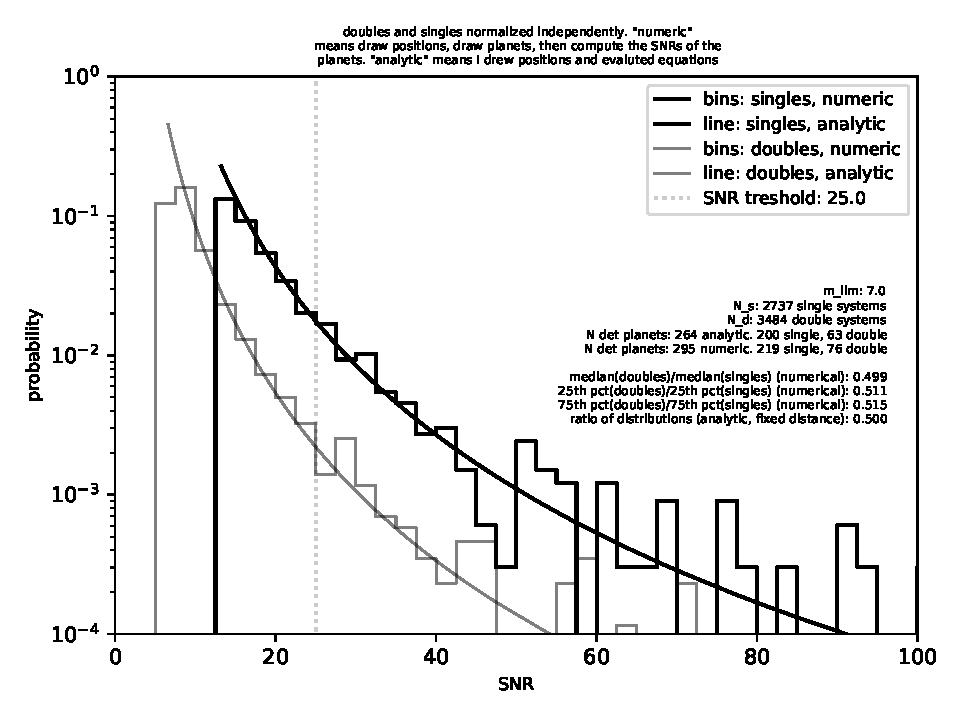
\includegraphics[scale=0.4]{figures/snr_distribution.pdf}
	\end{center}
	\caption{Comparison of analytic and numeric probability 
	density functions of the SNR in an idealized transit survey.
	The analytic lines are Eqs.~\ref{eq:prob_xs} and~\ref{eq:prob_xd} for the 
	planet populations orbiting single and binary stars. The underlying stepped 
	histogram is output from Monte Carlo simulations. Poisson noise leads to 
	a small deviation at the faint and bright limits, but the numerics and 
	analytics otherwise agree.
		 }
	\label{fig:snr_dist_analytic_v_numeric}
\end{figure}


\subsection{Representative numbers for a few cases}

\subsubsection{Twin binaries: if we ignore binarity, for what fraction of 
detections do we misclassify the radii?}
 
Ignoring binarity, we will detect $N_{\rm det,s}$ planets around single stars, 
and $N_{\rm det,d}$ planets around double stars. The latter set will be assumed 
to have radii $R_p \sqrt{\mathcal{D}}$.
The fraction of detections with misclassified radii can then be written
\begin{equation}
\frac{N_{\rm det,d}}{N_{\rm det,s} + N_{\rm det,d}} = \frac{1}{1+\alpha},
\end{equation}
for
\begin{equation}
\alpha \equiv \frac{1}{2({\rm BF})} (1+\gamma_R)^{3/2} 
\frac{\Gamma_{t,s}}{\Gamma_{t,d}}.
\end{equation}

For the nominal G2V dwarf case of ${\rm BF}=0.45$, twin binaries with equal 
occurrence rates this produces a misclassification rate of $24\%$, in agreement 
with Fig.~\ref{fig:snr_dist_analytic_v_numeric}.

\subsubsection{Twin binaries: if we ignore binarity, how wrong is our
occurrence rate for planets of radius $R_p$?}

This is almost simply asking ``what is the relative difference between the 
occurrence rates derived by Astronomers D and A for planets of radius $R_p$?''
However, in the more realistic case, Astronomer A also has derived a 
completeness, which we assume is the same as for Astronomer D in the single 
star case.
So Astronomer A now misclassifies planetary radii, and miscounts the total 
number of stars, but knows his completeness for single stars.
Astronomer D corrects all these errors.
Then
\begin{equation}
\Gamma_{{\rm A}, R_p} = \frac{N_{\rm det,s}/(f_{s,g} f_{s,c})}{N_s + N_d},
\end{equation}
and the relative difference between the two occurrence rates is

\begin{align}
\left|\frac{\Gamma_{{\rm A},R_p} - \Gamma_{{\rm D},R_p}}
		   {\Gamma_{{\rm A},R_p}} \right| &=
\left| 1 - \frac{\Gamma_{{\rm D},R_p}}{\Gamma_{{\rm A},R_p}}\right| \\
&=
\left| 1 - \left(\frac{\Gamma_{t,s}N_s + 2\Gamma_{t,d}N_d}{N_s + 2N_d}  \cdot 
\frac{N_s + N_d}{\Gamma_{t,s} N_s }\right)\right| \\
&= 
\left|
1 - \frac{(1 + 2 \beta \Gamma_{t,d}/\Gamma_{t,s})(1 + \beta)}{(1+2\beta)}
\right|,
\end{align}
for
\begin{equation}
\beta \equiv N_d/N_s = {\rm BF} \times (1+\gamma_R)^{3/2}.
\end{equation}

For the nominal G2V dwarf case of ${\rm BF}=0.45$ with twin binaries ($\gamma_R 
= 1$) and $\Gamma_{t,d} = \Gamma_{t,s}$ this gives a relative error of $127\%$.
For instance, in the numerical simulation corresponding to 
Fig.~\ref{fig:snr_dist_analytic_v_numeric}, Astronomer A finds $\Gamma_{\rm 
A,R_p} = 0.22$, while Astronomer 
D derives the true (input) occurrence rate of $\Gamma_{\rm D,R_p} = 0.5$.




\section{Model \#2: fixed stars, fixed planets, varying light-ratio binaries}
\label{sec:model_2}

Same story as Model \#1, except now $\gamma_R$ varies across the population 
of star systems.
It does so because the underlying mass ratio varies. 
Since we are interested in solar type binaries, we take the distribution of the 
mass ratio $q=M_2/M_1$ by approximating [Rhagavan et al 2010, Fig 16]:
\begin{equation}
{\rm prob}(q) =
\Bigg\{\begin{array}{lr}
c_q & 0.1 < q \leq 1  \\
0 & {\rm otherwise},
\end{array}
\label{eq:mass_ratio}
\end{equation}
for $c_q = 1/9$ to normalize the distribution to 1.
The mass-luminosity relation can, for analytic convenience, be approximated as 
$L = M^\alpha$, with the lore-value of $\alpha$ being $3.5$.
While we use this in subsequent analytic development, for numerics we fit a 
lines to mass-luminosity data collected by Torres et al. [2009] for 
dwarfs above M, and Benedict et al. [2016] for dwarfs below M.
To convert Benedict et al. [2016]'s reported $M_V$ values to absolute 
luminosities, we interpolated over E. Mamajek's 
table\footnote{
	\texttt{pas.rochester.edu/\textasciitilde 
		emamajek/EEM\_dwarf\_UBVIJHK\_colors\_Teff.txt},
	downloaded 2017.08.02}.
In log-log space, we let the intersection point of the lines float, and make 
various cuts on the data as indicated in Fig~\ref{fig:mass_luminosity}. The 
fit parameters are available in a footnote\footnote{
	m lo: 1.8818719873988132~--~
	c lo: -0.9799647314108376~--~
	m hi: 5.1540712426599882~--~
	c hi: 0.0127626185389781~--~
	M at merge: 0.4972991257826812~--~
	L at merge: 0.0281260412126928.
}.
\begin{figure}
	\begin{center}
		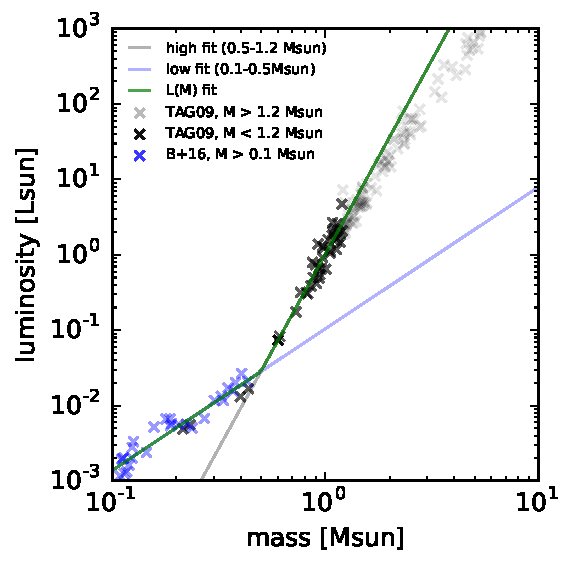
\includegraphics[scale=0.9]{figures/mass_luminosity.pdf}
	\end{center}
	\caption{Empirical fit to main sequence dwarf mass luminosity data from 
		Torres et al. [2009] and Benedict et al. [2016]. The ``low fit'' is a 
		least 
		squares fit to data from $0.1-0.5M_\odot$, and the ``high fit'' is to 
		data 
		above that, and below the Kraft break ($1.2M_\odot$).
		The $L(M)$ relation taken for subsequent numerics is the maximum 
		of the two fits.
	}
	\label{fig:mass_luminosity}
\end{figure}

The other changes between Model \#2 and Model \#1 are:
\begin{enumerate}
\item We allow a third occurrence rate, splitting $\Gamma_{t,d} \rightarrow 
(\Gamma_{t,d1}, \Gamma_{t,d2})$ where the latter terms represent the occurrence 
rate around the primary of a double star system, and the occurrence rate around 
the secondary of a double star system. For the case of \textit{e.g.}, $q=0.1$, 
this seems more relevant.
We can then take the limit that says ``any planet around the secondary is as 
likely as around the primary'', or go to the opposite extreme of ``there are 
only planets around the primaries, not the secondaries''.
%
\item Our binary systems have secondaries with varying masses. Thus they have 
varying radii. Taking [Demircan \& Kahraman 1991]'s empirical fit to eclipsing 
binary data,
\begin{equation}
R = 1.06 M^{0.945}
\label{eq:mass_radius}
\end{equation}
for all the stars in our desired mass range ($M < 1.66M_\odot$, D\&K 1991's 
stated bounds), and for each in solar units. This only affects the transit 
probabilities about the secondaries of binary star systems.
\end{enumerate}

We then ask the same questions as for Model \#1.

\subsection{How many stars are in the sample?}

Let $N_s$ be the number of single star systems, and $N_d$ the number of double 
star systems. $N_s$ is the same as in Sec.~\ref{sec:model_1}.

Now
\begin{equation}
N_d(\gamma_R) = n_d \frac{4\pi}{3} d_{\rm max,d}^3(L_1^N, \gamma_R, F_{\rm 
	lim}^N)
\end{equation}
for
\begin{equation}
d_{\rm max,d}(L_1^N, \gamma_R, F_{\rm lim}^N) =
d_{\rm max,s}(L_1^N, F_{\rm lim}^N)\times (1+\gamma_R)^{1/2}.
\end{equation}
Since $q$ is a random variable, $\gamma_R$ is a random variable, and $d_{\rm 
	max,d}$ is a random variable. Since $N_d$ is a function of $d_{\rm max,d}$, 
the number of double star systems becomes a random variable.
The expected (mean) number of double star systems in the sample is
\begin{equation}
\langle N_d \rangle = \int_{0}^{\infty} N_d\, {\rm prob}(N_d) \,{\rm d}N_d.
\end{equation}
By applying the chain rule for probability density functions, the distribution 
${\rm prob}(N_d)$ can be written 
\begin{equation}
{\rm prob}(N_d) = {\rm prob}(q(\gamma_R)) 
\left| \frac{{\rm d}q}{{\rm d}\gamma_R}  \right|
\left| \frac{{\rm d}\gamma_R}{{\rm d}d_{\rm max,d}}  \right|				
\left| \frac{{\rm d}d_{\rm max,d}}{{\rm d}N_d}  \right|.
\end{equation}
Doing some algebra, and assuming $\gamma_R = q^3$, this can be shown to be
\begin{align}
{\rm prob}(N_d) = \frac{2}{81} &N_d^{-1/3} \left(\frac{3}{4\pi 
	n_d}\right)^{2/3} d_{\rm max,s}^{-2/3} \ \times \nonumber\\
&\left[ \left(\frac{3 N_d}{4\pi n_d}\right)^{2/3} - d_{\rm 
	max,s}^2 \right]^{-2/3}
\end{align}
over the interval
\begin{equation}
{\rm lower\ bound} = \frac{4 \pi n_d}{3} (\sqrt{0.1^3 + 1} d_{\rm max,s})^3
\end{equation}
\begin{equation}
{\rm upper\ bound} = \frac{4 \pi n_d}{3} (\sqrt{2}d_{\rm max,s})^3,
\end{equation}
and outside the stated interval ${\rm prob}(N_d) = 0$.

While a closed analytic expression for $\langle N_d \rangle$ does exist, it is 
messy, and it does not yield much intuition. Instead, summarizing the important 
points and supporting them numerically:
\begin{itemize}
	\item In a volume-limited sample of binary star systems in which the 
	primary mass is fixed, and the mass ratio is drawn from a bounded uniform 
	distribution, the distribution of $\gamma_R$ will be biased towards low 
	values ($\gamma_R \approx 0.1$). This is shown in 
	Fig.~\ref{fig:gammaR_distribn_vol_limited}.
	\item In a magnitude-limited sample of binary star systems in which the 
	primary mass is fixed, and the mass ratio of the \textit{population} is 
	drawn from a bounded uniform distribution, the observed distribution of 
	mass ratios will be biased towards high values. You will see more twins,
	because they are detectable out to a greater distance\footnote{This is a 
	scarcy systematic w.r.t. the claimed intrinsic excess of twin binaries.}. 
	This is shown in 
	Fig.~\ref{fig:q_distribn_mag_limited}.
	\item In a magnitude-limited sample of binary star systems in which the 
	primary mass is fixed, the distribution of $\gamma_R$ will be biased 
	towards low values ($\approx 0.1$), but less so than in a 
	volume-limited sample. This is shown in 
	Fig.~\ref{fig:gammaR_distribn_mag_limited}.
\end{itemize}

In passing, the bias in ${\rm prob}(\gamma_R)$ towards low luminosity ratios 
can be seen analytically. If we assume $\gamma_R = q^\alpha$, then
\begin{equation}
{\rm prob}(\gamma_R) = \frac{1}{9 \alpha} \ \gamma_R^{\frac{1-\alpha}{\alpha}}
\quad {\rm for\ } (0.1)^\alpha < \gamma_R < 1,
\end{equation}
and otherwise zero. For instance if $\alpha = 3$, ${\rm prob}(\gamma_R) 
\propto \gamma_R^{-2/3}$ and the domain extends from $1$ to 
$10^{-3}$, where the probability distribution peaks.

\begin{figure}[!t]
	\begin{center}
		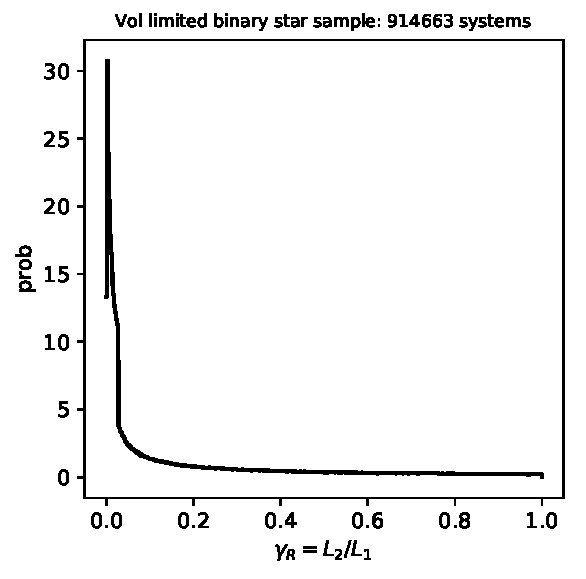
\includegraphics[scale=.8]{figures/gammaR_distribn_vol_limited.pdf}
	\end{center}
	\caption{The distribution of the luminosity ratio for a volume limited 
		sample of binary stars. ${\rm BF} = 0.45$ [Duchene and Kraus 2013]; 
		total 
		number density from Bovy 2017; $M(L)$ relation from 
		Fig.~\ref{fig:mass_luminosity}; mass ratios are drawn from 
		Eq.~\ref{eq:mass_ratio}.}
	\label{fig:gammaR_distribn_vol_limited}
\end{figure}
\begin{figure}[!t]
	\begin{center}
		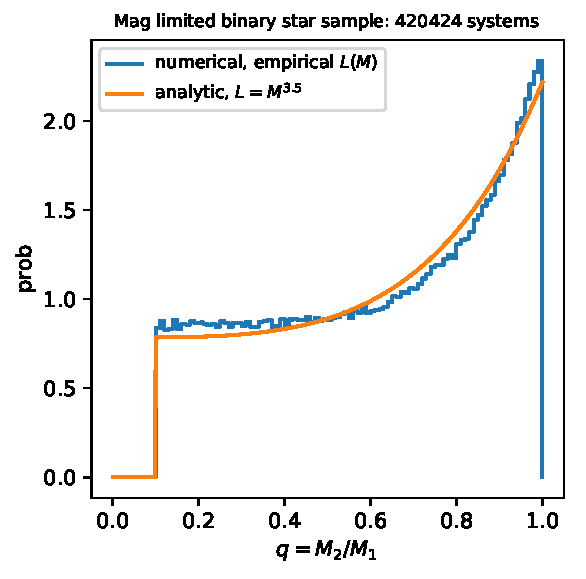
\includegraphics[scale=.8]{figures/q_distribn_mag_limited.pdf}
	\end{center}
	\caption{The distribution of the mass ratio for a magnitude limited 
		sample of binary stars. ${\rm BF} = 0.45$ [Duchene and Kraus 2013]; 
		total 
		number density from Bovy 2017; $M(L)$ relation from 
		Fig.~\ref{fig:mass_luminosity}; mass ratios are drawn from 
		Eq.~\ref{eq:mass_ratio} -- a \textit{uniform} distribution in a 
		volume-limited sample!}
	\label{fig:q_distribn_mag_limited}
\end{figure}
\begin{figure}[!t]
	\begin{center}
		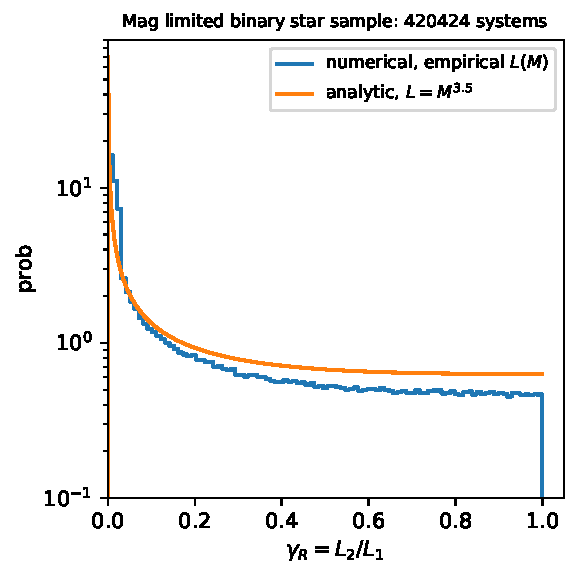
\includegraphics[scale=.8]{figures/gammaR_distribn_mag_limited.pdf}
	\end{center}
	\caption{The distribution of the luminosity ratio for a magnitude limited 
		sample of binary stars. ${\rm BF} = 0.45$ [Duchene and Kraus 2013]; 
		total 
		number density from Bovy 2017; $M(L)$ relation from 
		Fig.~\ref{fig:mass_luminosity}; mass ratios are drawn from 
		Eq.~\ref{eq:mass_ratio}.}
	\label{fig:gammaR_distribn_mag_limited}
\end{figure}

\paragraph{How many stars are in the sample?}

We return to the original question: how many stars?
\begin{equation}
\langle N_{\rm stars} \rangle = N_s + 2 \langle N_d \rangle,
\end{equation}
as before.
Since we are not giving analytic expressions for either of the $\langle \ldots 
\rangle$ terms, we just note that in the case of a population with a single 
$\gamma_R$ value, $N_d/N_s = {\rm BF} \times (1 + \gamma_R)^{3/2}$. A lower
bound for this ratio will always be the binary fraction.
For a single run of a Monte Carlo code, where ${\rm mean}(\gamma_R) = 0.28$, 
${\rm median}(\gamma_R) = 0.13$, and the distribution was that given in 
Fig.~\ref{fig:gammaR_distribn_mag_limited}, the observed ratio was $N_d/N_s = 
0.59$.
This corresponds to a single-valued population with $\gamma_R \sim 0.20$, a
number between the mean and median of the true distribution.
It means $\sim 1.2$ stars in binary star systems for every star in a single 
star system from this sample.

We also note in passing that $N_d/N_s = 0.59$ is a smaller ratio than for the 
case of a fixed $\gamma_R$ population with $\gamma_R = 1$, which gave $N_d/N_s 
= 1.27$. The difference is that in the latter population, the volume of 
searchable stars is greater. Based on the fixed-$\gamma_R$ population scaling 
law $N_d / N_s \propto (1+\gamma_R)^{3/2}$, we 
would expect the ratio of single stars to be $\sim (2/1.1)^{3/2} = 2.4$ 
times smaller, which is roughly (though not exactly) what we observe.



\subsection{How many planets are in the sample?}

The mean number of planets in the sample is
\begin{align}
\langle N_{\rm planets} \rangle
=& N_{\rm planets\ in\ single\ star\ systems}  +  \\
&\quad\quad N_{\rm planets\ in\ double\ star\ systems} 
\nonumber \\
=& \Gamma_{t,s} N_s + (\Gamma_{t,d1} + \Gamma_{t,d2}) \langle N_d \rangle.
\end{align}

What was formerly a factor of 2 has now been split into the true occurrence 
rates about the primaries and secondaries of double star systems.

\subsection{What is the true occurrence rate?}

The ``true occurrence rate'' is the average number of planets per star. Thus

\begin{align}
\Gamma_t &= \frac{\langle N_{\rm planets}\rangle}{\langle N_{\rm stars} 
\rangle} \\
\Gamma_t &= \frac{\Gamma_{t,s} N_s + (\Gamma_{t,d1} + \Gamma_{t,d2}) \langle 
N_d\rangle}{N_s +	2\langle N_d\rangle}.
\label{eq:true_occ_2}
\end{align}



\subsection{How many planets are detected?}

The total number of planet detections is the sum of the number of planets 
detected in single star systems $N_{{\rm det},s}$ and the number of planets 
detected in double star systems $N_{{\rm det},d}$.
The latter of these is a random variable, and can be further split into the 
primary and secondary contributions $N_{{\rm det},d1}$, $N_{{\rm det},d2}$.

The number of planets detected in single star systems is
\begin{equation}
N_{{\rm det},s} = N_s \Gamma_{t,s} f_{s,g} f_{s,c},
\end{equation}
where the product $N_s \Gamma_{t,s}$ is the number of planets in the single 
star systems of the sample, $f_{s,g}$ is the geometric probability of the 
planets transiting, and $f_{s,c}$ is the fraction of transiting planets around 
single star systems that are detected (the completeness).


The mean number of planets detected in double star systems is
\begin{equation}
\langle N_{{\rm det},d}\rangle = \langle N_d\rangle  
(\Gamma_{t,d1} f_{d1,g} f_{d1,c} + 
\Gamma_{t,d2} f_{d2,g} f_{d2,c} ).
\label{eq:N_det_d_2}
\end{equation}
Now $\langle N_d\rangle  \Gamma_{t,d1}$ is the mean number of planets orbiting 
the primaries of double star systems, ditto the corresponding expression for 
the secondaries.
For this population, $f_{d1,g} = f_{s,g}$, but $f_{d1,g} \neq f_{d2,g}$.
The completeness fractions differ between the primary and secondary because 
the dilution as a function of the light ratio, $\mathcal{D}(\gamma_R)$, has 
different behavior for the two cases.
We show this in Fig.~\ref{fig:rad_vs_gammaR}.
Specifically, a planet orbiting the secondary will have worse dilution than a 
planet orbiting the primary, and consequently lower completeness.

\begin{figure}[!t]
	\begin{center}
		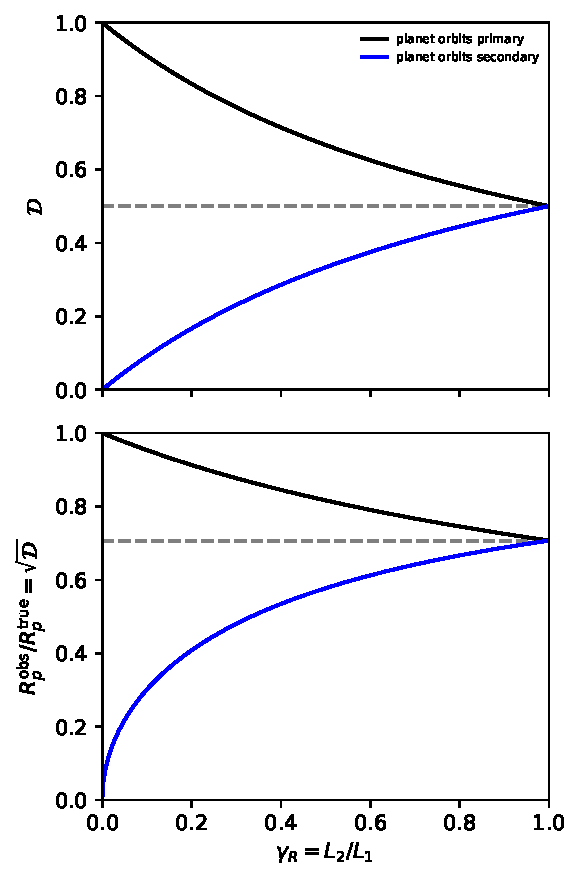
\includegraphics[scale=.9]{figures/observed_radii_vs_gammaR.pdf}
	\end{center}
	\caption{Dilution $\mathcal{D}$ and observed to true radius ratio 
	$\sqrt{\mathcal{D}}$ plotted against binary light ratio $\gamma_R$. This 
	illustrates	Eq.~\ref{eq:dilution}. The lower panel's horizontal line is at 
	$1/\sqrt{2}$.
	The implication is that if a detected planet orbits the secondary and you do 
	not know it, you cannot measure $R_p$ to better than $\approx 29\%$ 
	accuracy.
	Conversely, if it orbits the primary and you do not know it, you will get 
	the radius wrong by at most $\approx 29\%$.
	}
	\label{fig:rad_vs_gammaR}
\end{figure}

We could probably derive analytic expressions for all the terms between 
brackets in Eq.~\ref{eq:N_det_d_2}, completeness included.
I'm not yet convinced we need to -- we should get cancellations for
most of the questions we want to ask.

\subsubsection{Analytic completeness}
\texttt{todo, if necessary}
\subsubsection{Deriving ${\rm prob}(x_i)$}
\texttt{todo, if necessary}
\subsubsection{Number of detected planets}
\texttt{todo, if necessary}

\subsection{Astronomer A ignores binarity}

Just as in Sec.~\ref{sec:model_1}, Astronomer A
\begin{itemize}
\item has never heard about binary star systems.
\item has never heard about completeness corrections.
\item knows about geometric transit probabilities.
\end{itemize}

What occurrence rate does he derive for planets of radius $R_p$ and period $P$?

The answer is the same as in Sec.~\ref{sec:model_1},
\begin{equation}
\Gamma_{{\rm A}, R_p} = \frac{N_{\rm det,s}/f_{s,g}}{N_s + N_d}.
\end{equation}

However, now rather than planets detected in binary systems being perceived as 
a second population of planets with fixed radius $R_p \sqrt{\mathcal{D}}$, 
there will be an apparent spectrum of diluted radii, since $\mathcal{D}$ 
varies by system.
Writing the number of detections in double systems as a function of observed 
radius, $N_{\rm det,d}(R_p^{\rm obs})$, Astronomer A would derive an 
occurrence rate for this separate population of
\begin{equation}
\Gamma_{\rm A}(R_p^{\rm obs}) = \frac{N_{\rm det,d}(R_p^{\rm 
obs})/f_{s,g}}{N_s + N_d}.
\end{equation}
Note that this astronomer thinks these planets orbit single stars, 
and so miscomputes the geometric transit probability for the secondaries.

A more realistic question is ``what fraction of multiples have $\gamma_R$ 
smaller enough so that you'd still observe a radius close to the true one?''. 
We discuss this in Sec.~\ref{sec:close_enough}.

\subsection{Astronomer B counts host stars correctly}

Same as astronomer A above, except the denominator becomes $N_s + 2N_d$.

\subsection{Astronomer C counts host stars correctly and figures out diluted
radii}

In Sec.~\ref{sec:model_1}, Astronomer C only had to do high resolution 
imaging to measure $\gamma_R$ for each system. Since for $\gamma_R = 1$, the 
dilution is single-valued (Fig.~\ref{fig:rad_vs_gammaR}), this immediately 
told her the true planet radius (since the primary/secondary distinction was 
meaningless).

In Model \#2's universe, the dilution is double-valued for a given $\gamma_R$.
To correctly work out the diluted radii, Astronomer C now needs more than high 
resolution imaging -- she needs to resolve the stars during transit to 
discover which star the planet orbits.
She also needs to derive masses for the primaries and secondaries (to make the 
geometric transit probability correction).

Only after doing this does she find that all detected planets from this survey 
have radii $R_p$. She computes an occurrence rate
\begin{equation}
	\Gamma_{{\rm C},R_p} = 
	\frac
			{N_{\rm det,s}/f_{s,g} +
			  N_{\rm det,d1}/f_{d1,g} +
			  N_{\rm 	det,d2}/f_{d2,g}}
			{N_s + 2N_d}
\end{equation}

the closest yet to the true rate (Sec.~\ref{sec:true_rate}).


\subsection{Astronomer D counts host stars correctly, figures out diluted
radii, and accounts for completeness}

Same story as for Model \#1.
Now, they do injection recovery and derive correct estimates for their 
completeness functions about single stars $f_{s,c}$, the primaries of double 
star systems, $f_{d1,c}$, and the secondaries of double star systems 
$f_{d2,c}$.
They compute the respective single and binary 
occurrence rates
\begin{equation}
\Gamma_{t,s} = \frac{N_{\rm det,s}}{N_s f_{s,g} f_{s,c}},
\end{equation}
\begin{equation}
\Gamma_{t,d1} = \frac{N_{\rm det,d1}}{N_d f_{d1,g} f_{d1,c}},
\end{equation}
\begin{equation}
\Gamma_{t,d2} = \frac{N_{\rm det,d2}}{N_d f_{d2,g} f_{d2,c}}.
\end{equation}

With these in hand, they derive the overall occurrence rate
\begin{align}
\Gamma_{{\rm D}, R_p} 
&= \frac{
	N_{\rm det,s}/f_s + 
	N_{\rm det,d1}/f_{d1} +
	N_{\rm det,d2}/f_{d2}
	}
	{N_s + 2 N_d} \\
&= \frac{\Gamma_{t,s} N_s + (\Gamma_{t,d1} + \Gamma_{t,d2})N_d}
				{N_s + 2 N_d},
\end{align}
where $f_s \equiv f_{s,g}f_{s,c}, f_{d1} \equiv f_{d1,g}f_{d1,c}, 
f_{d2} \equiv f_{d2,g}f_{d2,c}$ for brevity.
Astronomer D's occurrence rate is the true occurrence rate (cf. 
Eq.~\ref{eq:true_occ_2}).


\subsection{Numerical verification}
\texttt{todo, if needed}


\subsection{Representative numbers for a few cases}

We have not given analytic expressions for the number of double star systems 
$N_d$ because even with simplified $M(L)$ relations, they are unwieldy.
However, we can ask similar numerical questions as from Sec.~\ref{sec:model_1}, 
and compare the answers.


\subsubsection{If we ignore binarity, for what fraction of detections do we
misclassify the radii?}

Ignoring binarity, we will detect $N_{\rm det,s}$ planets around single stars, 
and $N_{\rm det,d}$ planets around double stars. The latter set will be assumed 
to have radii $R_p \sqrt{\mathcal{D}}$, where $\mathcal{D}$ is the vector of 
dilutions appropriate for each binary star system.
The fraction of detections with misclassified radii can then be written
\begin{equation}
\frac{N_{\rm det,d}}{N_{\rm det,s} + N_{\rm det,d}} = \frac{1}{1+\alpha},
\end{equation}
for
\begin{equation}
\alpha \equiv 
\frac{ N_d (\Gamma_{t,d1} f_{d1} + \Gamma_{t,d2} f_{d2}) }{N_s \Gamma_{t,s} 
f_s},
\end{equation}
where $f_s \equiv f_{s,g}f_{s,c}, f_{d1} \equiv f_{d1,g}f_{d1,c}, 
f_{d2} \equiv f_{d2,g}f_{d2,c}$ for brevity.

% For the nominal G2V dwarf case of ${\rm BF}=0.45$, and the same distributions 
% used to generate 
% Figs.~\ref{fig:gammaR_distribn_vol_limited}~--~\ref{fig:gammaR_distribn_mag_limited},
% we found $N_d/N_s=0.59$.
% We are assuming $\Gamma_{t,d} / \Gamma_{t,s} = 1$.
% If we maintained the (incorrect) assumption that $f_{d,{\rm geom}} / f_{s,{\rm 
% 		geom}} = 1$, this would give a misclassification rate of 45\%. 
% 
% This latter assumption is wrong because although we are letting the occurrence 
% rate be the same across binary and single systems, our binary systems have 
% secondaries with varying masses. Thus they have varying radii.
% Taking [Demircan \& Kahraman 1991]'s empirical fit to eclipsing binary data,
% \begin{equation}
% R = 1.06 M^{0.945}
% \label{eq:mass_radius}
% \end{equation}
% for all the stars in our desired mass range ($M < 1.66M_\odot$, D\&K 1991's 
% stated bounds).
% For a zero eccentricity system, $f_{\rm geom}=R_\star/a$.
% Since $f_{d,{\rm geom}} = 0.5\times (f_{d1,{\rm geom}} + f_{d2,{\rm geom}})$, 
% \textit{i.e.} it is the average of the transit probabilities for both the 
% primary and secondary (d1 and d2), we can write (dropping the ``geom'' 
% subscript)
% \begin{align}
% \frac{f_d}{f_s} &= \frac{1}{2} \left(1 + \left(\frac{M_1}{M_{d2}}\right)^{1/3} 
% \frac{R_{d2}}{R_1}\right) \\
% &= \frac{1}{2} \left( 1 + q^{-1/3 + 0.945}\right).
% \end{align}
% 
% Computing it all out in a numerical simulation, the only thing that changes 
% analytically is that
% \begin{equation}
% N_d f_d \rightarrow \sum_{i=1}^{N_d} f_{d,i},
% \end{equation}
% so when considering the ratio $f_d/f_s$, we are in fact interested in
% \begin{equation}
% \frac{\langle f_d \rangle}{f_s} = \frac{\frac{1}{N_d} \sum_{i=1}^{N_d} 
% 	f_{d,i}}{f_s},
% \end{equation}
% where $f_{d,i}$ is the vector of geometric transit probabilities across all 
% systems.
% For the same numerical realization with $N_d/N_s = 0.59$, and using the mass 
% radius relation given by Eq.~\ref{eq:mass_radius}, I get $\langle f_d 
% \rangle / f_s = 0.84$ (smaller secondaries lead to a smaller average transit 
% probability in double star systems), for a radius misclassification rate of 
% $0.51$.


\texttt{The different secondary completeness matters here if proceeding 
analytically. Would be easier to do numerically.
Regardless, this is not the most interesting question right now.}

\subsubsection{If we ignore binarity, how wrong is our occurrence rate for
planets of radius $R_p$?}

Write $\Gamma_{{\rm A,\ planets\ of\ }R_p} = \Gamma_{{\rm A,}R_p}$, 
and similarly for ${\rm D}$.
Just as in Model \#1, the answer to ``what is the relative difference between 
the occurrence rates derived by Astronomers D and A for planets of radius 
$R_p$?''
is simpler when we assume that Astronomer A has also derived a 
completeness, which we assume is the same as for Astronomer D in the single 
star case.
So Astronomer A now misclassifies planetary radii, and miscounts the total 
number of stars, but knows his completeness for single stars.
Astronomer D corrects all these errors.
Then
\begin{equation}
	\Gamma_{{\rm A}, R_p} = \frac{N_{\rm det,s}/(f_{s,g} f_{s,c})}{N_s + N_d}.
\end{equation}

The relative difference between the two occurrence rates, $\Delta \equiv 
\left|(\Gamma_{{\rm A},R_p} - \Gamma_{{\rm D},R_p})/\Gamma_{{\rm A},R_p} 
\right|$, is
\begin{align}
	\Delta &=
	\left| 1 - \frac{\Gamma_{{\rm D},R_p}}{\Gamma_{{\rm A},R_p}}\right| \\
	&=
	\left| 1 - \left(\frac{\Gamma_{t,s}N_s + (\Gamma_{t,d1} + 
	\Gamma_{t,d2})N_d}{N_s + 2N_d}  
	\cdot 
	\frac{N_s + N_d}{\Gamma_{t,s} N_s }\right)\right| \\
	&= 
	\left|
	1 - \frac{(1 + \beta (\Gamma_{t,d1}+\Gamma_{t,d2})/\Gamma_{t,s})(1 + 
	\beta)}{(1+2\beta)}
	\right| \\
	&=
	\left| 1 - \left(
	\left[ 1 + \chi \beta \right]
	\cdot 
	\frac{1 + \beta}{1 + 2\beta }
	\right) \right|
\end{align}
for
\begin{equation}
\beta \equiv N_d/N_s, \quad \chi \equiv 
(\Gamma_{t,d1}+\Gamma_{t,d2})/\Gamma_{t,s}.
\end{equation}

In the limit where the $R_p$ planet has the same occurrence rate about every 
host type regardless of its mass, $\chi=2$, and this simplifies to $\Delta = 
\beta$, for a relative error of $59\%$.
This is less than for Model \#1 because of the smaller volume of searchable 
binary stars in Model \#2.

If we consider the opposite limit of the $R_p$ planet \textit{only} 
existing around single stars and the primaries of double star systems with 
equal occurrence, $\chi = 1$, and $\Delta = \beta^2 / (1+2\beta)$.
For $\beta = 0.59$, this gives $\Delta = 0.16$.




\subsubsection{What if we ignore binarity, but count derived planet radii that 
are ``close enough''?}
\label{sec:close_enough}

Let $x$ be the acceptable margin of error on the observed radius, so that we 
are interested in counting the number of planets detected with $R_p < R_p^{\rm 
obs} < (1\pm x) R_p$.
For Model \#2, since all planets have radius $R_p$, we only care about 
the smaller radius case, \textit{i.e.}, we want to count $R_p < R_p^{\rm 
	obs} < (1 - x) R_p$, for instance with $x=0.1$.

All of these diluted detections will be from binary systems. The number of 
planets detected in double star systems with observed radius $R_p^{\rm obs}$ 
is
\begin{align}
N_{\rm det,d}(R_p^{\rm obs}) &= N_{\rm det, d1}(R_p^{\rm obs}) + 
															  N_{\rm det, d2}(R_p^{\rm obs}) \\
&= \Gamma_{t,d1} f_{d1}(R_p^{\rm obs}) N_{d1}(R_p^{\rm obs})\  + \nonumber \\
&\quad\quad \quad\Gamma_{t,d2} f_{d2}(R_p^{\rm obs}) N_{d2}(R_p^{\rm obs}).
\end{align}
As always, the fractional terms $f_{di}$ for $i\in{1,2}$ encompass geometric 
and completeness corrections.
We're writing both them and the number of stars for which a given observed 
radius would be seen as functions of $R_p^{\rm obs}$.

To save on notational horribleness, write $R_p' \equiv \{(1-x) R_p < R_p^{\rm 
	obs} < R_p\}$, in other words let $R_p'$ denote the set of planets 
	that are observed in the desired radius range.

Then writing $N_{d1}(R_p')$ is relatively straight-forward:
\begin{equation}
N_{d1}(R_p') = \int_{0}^{{\rm min}(1,\gamma_{R,u})} N_d(\gamma_R) 
\,{\rm prob}(\gamma_R) \,{\rm d}(\gamma_R),
\end{equation}
where the upper limit is set by equating the limiting radius $(1-x)R_p$ to the 
observed diluted radius $(1+\gamma_R)^{-1/2}R_p$, giving
\begin{equation}
\gamma_{R,u} \equiv \frac{x (2-x)}{(1-x)^2}.
\end{equation}
If $x > (1 - 2^{-1/2})$, bad things happen (cf. Fig.~\ref{fig:rad_vs_gammaR}), 
hence the need for the minimum.

The analogous equation for secondaries is
\begin{equation}
N_{d2}(R_p') = 
  \Bigg\{\begin{array}{lr}
  \int_{\gamma_{R,l}}^{1} N_d(\gamma_R)
  \,{\rm prob}(\gamma_R) \,{\rm d}(\gamma_R),\\ 
  \quad\quad\quad\quad\quad\quad\quad\quad x > 1 - 
  2^{-1/2}\\
  0, \quad\quad\quad\quad\quad\quad\quad x \leq 1 - 2^{-1/2}
  \end{array}
\label{eq:N_Rp_secondary}
\end{equation}
where
\begin{equation}
\gamma_{R,l} \equiv \frac{(1-x)^2}{x (2-x)}.
\end{equation}
Eq.~\ref{eq:N_Rp_secondary} accounts for the fact that you cannot measure 
$R_p$ to better than $\approx 29\%$ if the planet orbits the secondary of an 
unidentified binary.
This was originally noted in Fig.~\ref{fig:rad_vs_gammaR}.

If we were forward-modelling (\textit{i.e.} we actually wanted to compute 
$N_{\rm det,d}(R_p')$) we would need to evaluate the completeness 
term and this ``fraction of slightly diluted stars'' terms together, and 
integrate jointly to find $N_{\rm det,d1}(R_p')$ and $N_{\rm det,d2}(R_p')$.

\texttt{If we ask the right question, this will not be necessary.}

Astronomer A misclassifies planetary radii, miscounts the total number of 
stars, but knows his completeness and geometric correction for single stars as 
a function of radius $f_s(R_p')$.
His occurrence rate for planets of radius \textit{near} $R_p$, \textit{i.e.} 
the set of planets with $\{ (1-x)R_p < R_p^{\rm obs} < R_p \}$, is
\begin{equation}
\Gamma_{{\rm A}, R_p'} = \frac{ (N_{\rm det,s} + N_{\rm det,d}(R_p')) 
/ f_s(R_p')   }{ N_s + N_d}.
\end{equation}

For him,
\begin{equation}
f_s(R_p') = f_{s,g}(R_p') f_{s,c}(R_p').
\end{equation}

Astronomer D, who had everything right, doesn't change anything.

The new difference between the two rates is
\begin{align}
\Delta' &\equiv \left|
\frac{\Gamma_{{\rm A},R_p'} - \Gamma_{{\rm D},R_p}}{\Gamma_{{\rm A},R_p'} }
\right| \\
&= \left|
1 - \frac{\Gamma_{{\rm D},R_p}}{\Gamma_{{\rm A},R_p'} } 
\right| \\
&=
\left| 1 -
\left( \frac{1+\chi \beta}{1 + \xi}  \cdot 
\frac{1 + \beta}{1 + 2\beta} \right)
\right|,
\end{align}
for
\begin{equation}
\beta \equiv N_d/N_s, \quad \chi \equiv (\Gamma_{t,d1} + 
\Gamma_{t,d2})/\Gamma_{t,s},
\end{equation}
and
\begin{equation}
\xi \equiv \frac{N_{\rm det,d}(R_p')}{f_s(R_p')} \cdot \frac{1}{N_s 
\Gamma_{t,s}}.
\end{equation}
If we let $x < 1 - 2^{-1/2}$, for instance $x=0.1$, then $N_{d2}(R_p') = 0$. 
The expression for $\xi$ simplifies to
\begin{equation}
\chi = \frac{N_{d1}(R_p')}{N_s} \cdot \frac{\Gamma_{t,d1}}{\Gamma_{t,s}} \cdot 
\frac{f_{d1}(R_p')}{f_s(R_p')},\quad ({\rm if\ }x < 1-2^{-1/2}).
\label{eq:chi_simplfied}
\end{equation}

If we assume $\Gamma_{t,d1} = \Gamma_{t,s}$, as we were doing 
anyway, Eq.~\ref{eq:chi_simplfied} is bounded above by
$\beta$. This is because $N_{d1}(R_p') \leq N_{d1} = N_d$, and $f_{d1}(R_p') / 
f_s(R_p') \leq 1$, since over a fixed radius interval dilution will always 
yield a lower completeness fraction for double star systems than singles.
Recall for the fixed $\gamma_R$ population we showed that $f_{d1}/f_s = 
(1+\gamma_R)^{-3}$.

Regardless, the cheap way of making the estimate without deriving the actual 
completeness fractions, or even running numerics, is just to plot the error as 
a function of $\xi$. We do this in Fig.~\ref{fig:deltaprime_vs_xi}, which 
shows that the
relative error varies between $\approx 5\% - 35\%$, depending on what 
fraction of secondaries you assume host planets.

\begin{figure}[!t]
	\begin{center}
		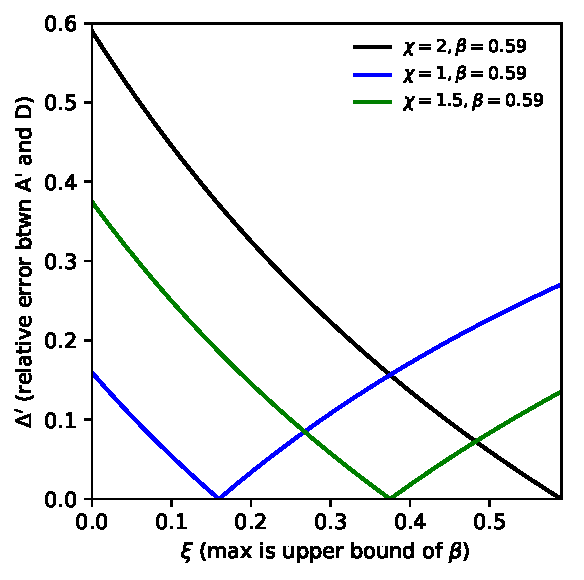
\includegraphics[scale=.8]{figures/deltaprime_vs_xi.pdf}
	\end{center}
	\caption{\textit{Y axis}: relative error between the Astronomer who ignores 
	binarity 
	but counts planetary radii that are ``close enough'' (A') and the Astronomer 
	who knows everything (D).
	\textit{X axis}: $\chi$ as defined in Eq.~\ref{eq:chi_simplfied}. Taking a 
	guess at the true value, if $N_{d1}(R_p') = N_d/2$, and the occurrence rates 
	between `d1' and `s' are the same, and we put $\gamma_R = 0.1$ into the 
	completeness ratio, then $\xi = (\beta/2) \times (1+0.1)^{-3} = 0.22$. The 
	relative error then varies between $\approx 5\% - 35\%$, depending on what 
	fraction of secondaries you assume host planets.
		}
	\label{fig:deltaprime_vs_xi}
\end{figure}



%FIXME

% \begin{comment}
% \subsection{How many stars are in the sample?}
% \subsection{How many planets are in the sample?}
% \subsection{What is the true occurrence rate?}
% \subsection{How many planets are detected?}
% \subsubsection{Analytic completeness}
% \subsubsection{Deriving ${\rm prob}(x_i)$}
% \subsubsection{Number of detected planets}
% \subsection{Astronomer A ignores binarity}
% \subsection{Astronomer B counts host stars correctly}
% \subsection{Astronomer C counts host stars correctly and figures out diluted
% radii}
% \subsection{Astronomer D counts host stars correctly, figures out diluted
% radii, and accounts for completeness}
% \subsection{Numerical verification}
% \subsection{Representative numbers for a few cases}
% \subsubsection{If we ignore binarity, for what fraction of detections do we
% misclassify the radii?}
% \subsubsection{If we ignore binarity, how wrong is our occurrence rate for
% planets of radius $R_p$?}
% \subsubsection{If we ignore binarity, but allow derived planet radii to be
% ``close enough'', how do we do?}
% 
% \end{comment}


\newpage

%\begin{thebibliography}{}


%\end{thebibliography}

\end{document}
